\documentclass{beamer}
\usepackage[utf8]{inputenc}

\usepackage{utopia} %font utopia imported
\usepackage{xcolor}
\usetheme{Boadilla}
\usecolortheme{beaver}

%------------------------------------------------------------
%This block of code defines the information to appear in the
%Title page
\title[] %optional
{On Dependency Analysis of NPM}

\subtitle{A Survey}

\author[Wang] % (optional)
{Guochang Wang\\dz1933026@smail.nju.edu.cn}

\institute[ICS] % (optional)
{
  Institute of Computer Software\\
  Nanjing University
}

\date[Report 2020.10] % (optional)
{I2EC Report, Oct 2020}

\logo{
\includegraphics[height=0.5cm]{nju_logo.png}}

%End of title page configuration block
%------------------------------------------------------------



%------------------------------------------------------------
%The next block of commands puts the table of contents at the 
%beginning of each section and highlights the current section:

\AtBeginSection[]
{
  \begin{frame}
    \frametitle{Sections}
    \tableofcontents[currentsection]
  \end{frame}
}
%------------------------------------------------------------


\begin{document}

%The next statement creates the title page.
\frame{\titlepage}


%---------------------------------------------------------
%This block of code is for the table of contents after
%the title page
\begin{frame}
\frametitle{Sections}
\tableofcontents
\end{frame}
%---------------------------------------------------------


\section{Background: NPM Dependency Hell}

%---------------------------------------------------------
%Changing visivility of the text
\begin{frame}
\frametitle{Node.js and Node Package Manager(NPM)}
\begin{figure}
    \centering
    
\includegraphics[height=0.4\textheight]{nodejs.png}
\end{figure}
\end{frame}

\begin{frame}
\frametitle{Node.js and Node Package Manager(NPM)}
\begin{columns}
\column{0.6\textwidth}
\begin{figure}
    \centering
    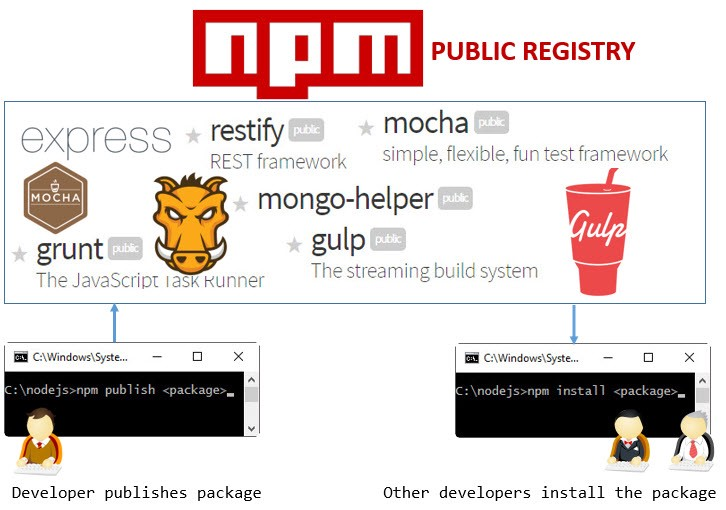
\includegraphics[width=\textwidth]{npm.jpeg}
\end{figure}
\column{0.4\textwidth}
\begin{figure}
    \centering
    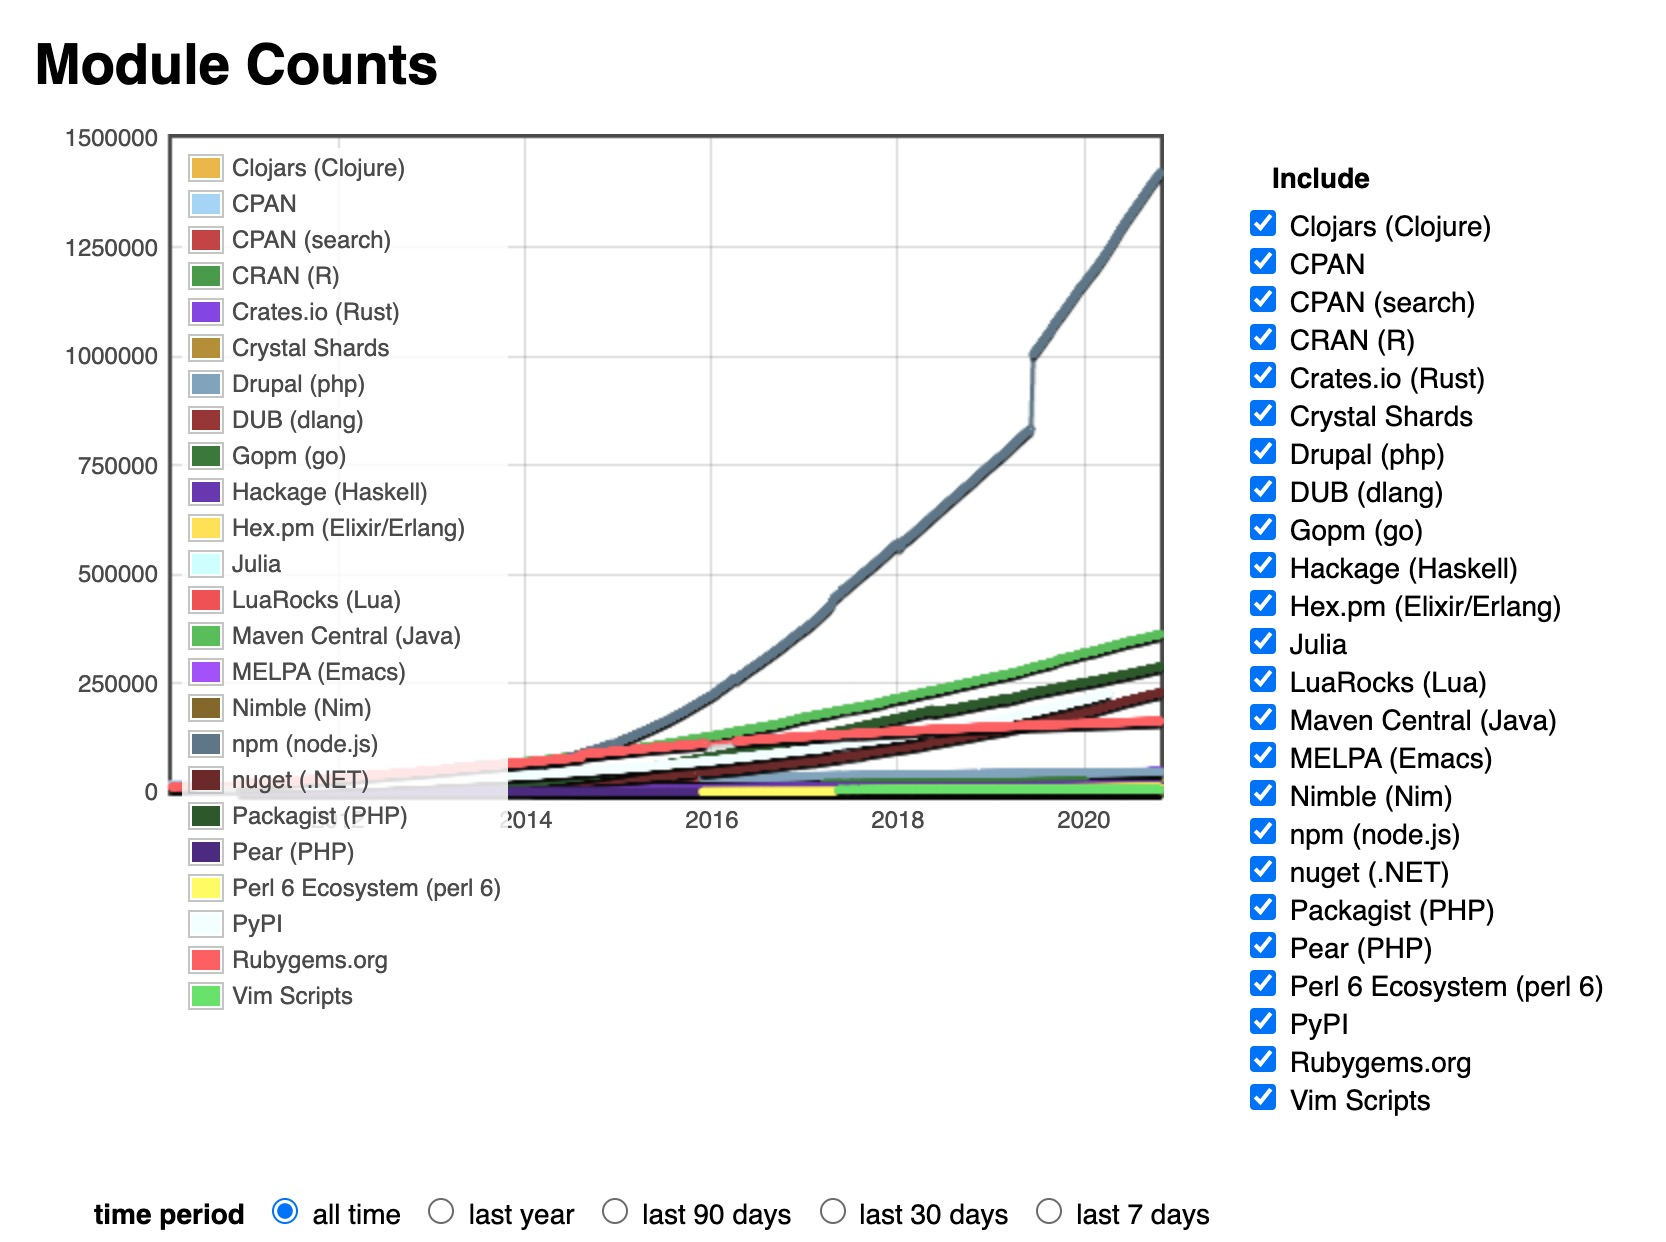
\includegraphics[width=\textwidth]{modulecount.jpg}
\end{figure}
\end{columns}

\end{frame}
%---------------------------------------------------------


%---------------------------------------------------------
%Example of the \pause command
\begin{frame}
\frametitle{NPM Dependency Hell\footnote{https://en.wikipedia.org/wiki/Dependency\_hell}}
\begin{block}{Definition}
The frustrating problems that occur when \textbf{a software package depends on several other packages}.
\end{block}
\begin{columns}
\column{0.6\textwidth}
\begin{itemize}
    \item Many dependencies
    \item Long chains of dependencies
    \item Conflicting dependencies
    \item Circular dependencies
    \item \textcolor{red}{Package manager dependencies}
    \item Diamond dependency
\end{itemize}
\column{0.4\textwidth}
\begin{figure}
    \centering
    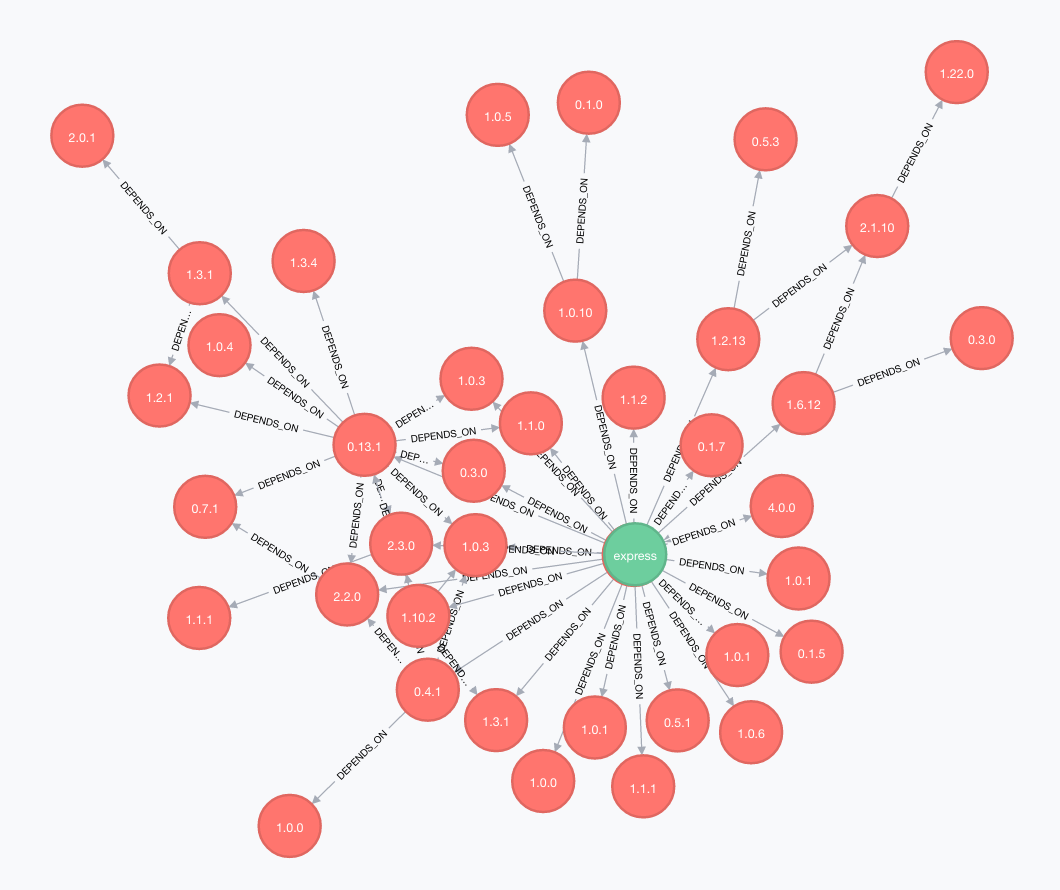
\includegraphics[width=\textwidth]{hell.png}
\end{figure}
\end{columns}
\end{frame}

\begin{frame}{NPM Dependency Hell: Representative Incident\footnote{https://www.infoworld.com/article/3047177/javascript/
how-one-yanked-javascript-package-wreaked-havoc.html}}
\begin{alertblock}{Left-Pad Incident}
Koçulu \alert{unpublished} a NPM package named "Left-Pad", causing all its downstream packages to \alert{crash} on installation, including \alert{Babel}(over 16,000 Dependents by 2020.10.22) and \alert{Webpack}(20,983 Dependents by 2020.10.22).
\end{alertblock}
Now developers are forbidden from abandoning packages directly. \\But vulnerable or malicious code in a single package may still affect thousands of others, e.g. through breaking API change.
\end{frame}
%---------------------------------------------------------

\section{Conflicting Threat Assessment: Small World with High Risks?}

%---------------------------------------------------------
%Highlighting text
\begin{frame}
\frametitle{Small World with High Risks: A Study of Security Threats in the npm Ecosystem\footnote{Small World with High Risks: A Study of Security Threats in the npm Ecosystem. USENIX Security 2019, Markus Zimmermann et al.}}
\begin{alertblock}{General Research Question}
Are these security incidents unfortunate individual cases or first evidence of a more general problem?
\end{alertblock}
\begin{columns}
\column{0.6\textwidth}
\textcolor{red}{Some Results}
\begin{itemize}
    \item Some highly popular packages reach more than 100,000
other packages, making them a prime target for attacks.
    \item Up to 40\% of 5,386,239 versioned packages rely on code known to be
vulnerable.
\end{itemize}
\column{0.4\textwidth}
\begin{figure}
    \centering
    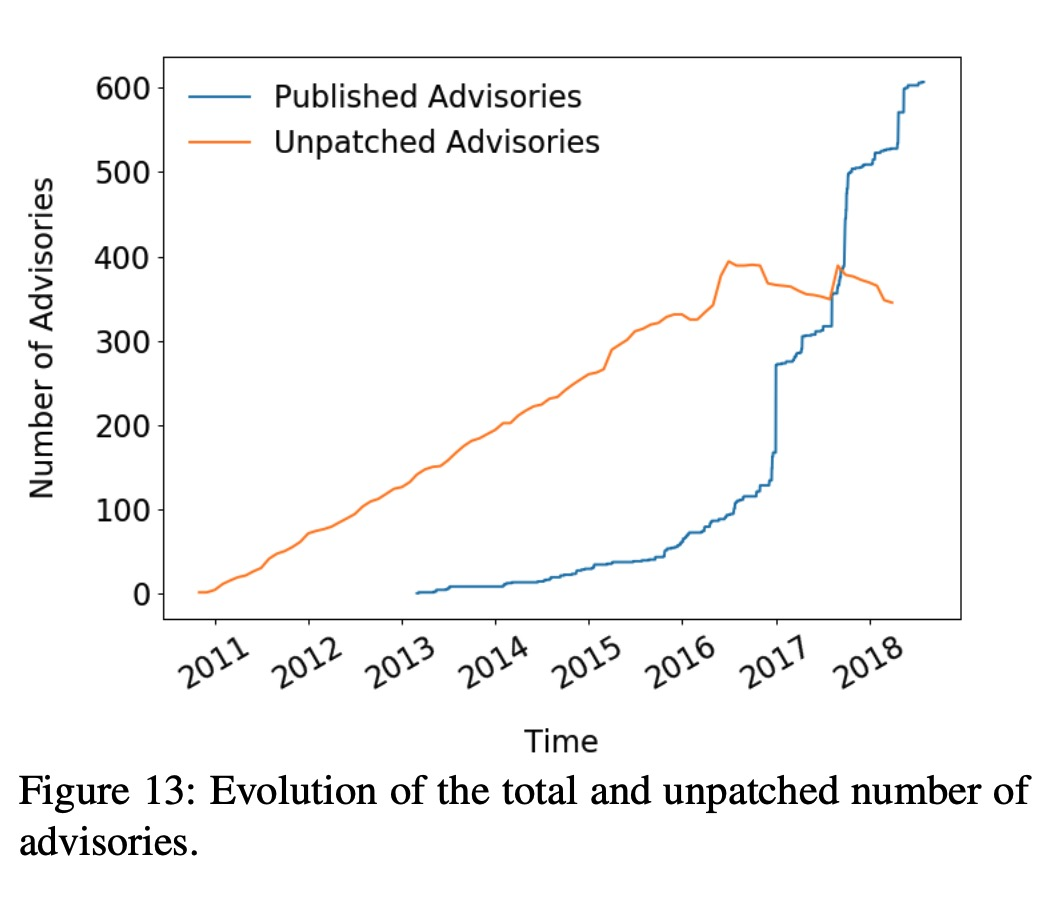
\includegraphics[width=\textwidth]{risk.jpg}
\end{figure}
\end{columns}
\end{frame}

\begin{frame}{Small World with \textbf{High} Risks?}
Mahmoud et al. conducted an empirical study involving 6,673 real-world, active, and mature open source Node.js applications.\footnote{On the Threat of npm Vulnerable Dependencies in Node.js Applications, arxiv, Mahmoud Alfadel et al.}
\begin{alertblock}{Core Insight}
Our experience leads us to believe that, in the grand scheme of things, these software vulnerabilities may have less impact than what is reported.
\end{alertblock}
\textcolor{red}{Conclusion}
The findings show that although 67.93\% of the examined applications
depend on at least one vulnerable package, 94.91\% of the vulnerable packages in those affected applications are classified as having
low threat. 
\end{frame}
%---------------------------------------------------------

\section{Get At the Truth: Methodology and Obstacles}
%---------------------------------------------------------
%Two columns
\begin{frame}{Which Study is the Truth?}
\begin{alertblock}{Threat to Validity}
Both of the studies conducted their analysis at package level. Based on hosted vulnerability databases, e.g. Snyk\footnote{https://snyk.io/}, Rapid7\footnote{https://www.rapid7.com/}, whose data is basically an aggregation of GitHub issues and bug reports from different package managers. 
\end{alertblock}
\pause
Essentially, the studies give same results based on different \textbf{assumptions}.
\begin{itemize}
    \item High Risk: if a package is vulnerable, then all it \textbf{dependents} are vulnerable.
    \item Low Threat: if a package is \textbf{not reported} as high threat, then it's \textbf{not vulnerable}.
\end{itemize}
\end{frame}


%---------------------------------------------------------

\begin{frame}{Function Call Graph: Concrete Methodology}
\textcolor{red}{Vulnerability Comes from Functions}: A package is vulnerable because of its \textbf{function(s)}, which you may \textbf{not} even called. 
\begin{alertblock}{Research Problem}
How to judge the correlation between vulnerability of a NPM project and its dependencies?
\end{alertblock}
A fine-grained dependency network that goes beyond packages and into call graphs is needed.
\end{frame}

\begin{frame}{Function Call Graph: Concrete Methodology}
Actually, various analysis methodologies based on JavaScript function call graph was proposed before.
\begin{itemize}
    \item Software Ecosystem Call Graph for Dependency Management, ICSE-NIER 18, Joseph et al.
    \item Towards Smoother Library Migrations: A Look at Vulnerable Dependency Migrations at Function Level for npm JavaScript Packages, ICSME 18, Rodrigo et al.
    \item Static analysis of event-driven Node.js JavaScript applications, SIGPLAN Notices 15, Magnus et al.
    \item Efficient construction of approximate call graphs for JavaScript IDE services, ICSE 13, Asger et al.
\end{itemize}
\end{frame}

\begin{frame}{Function Call Graph: Workflow\footnote{Impact Analysis of Cross-Project Bugs on Software Ecosystems, ICSE 20, Wanwangying Ma et al.}}
\begin{figure}
    \centering
    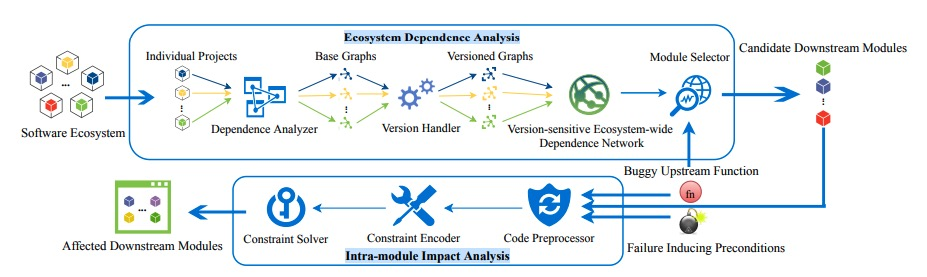
\includegraphics[width=\textwidth]{workflow.jpg}
\end{figure}
\end{frame}

\begin{frame}{Function Call Graph: Formalization}
\begin{block}{Formalization}
Denote $P$ as a package, $f$ as a function. We have $P = \{f_1,f_2,\dots,f_n\}$. \\
Denote $V = P_1\cup P_2\cup \dots \cup P_m$, which forms a vertex set.\\ $f_i$ has an edge to $f_j$ \textbf{iff.} $f_i$ calls $f_j$, recorded as $\langle f_i, f_j \rangle$.\\
Thus, an edge set can be represented as $E = \{ \langle f_i, f_j \rangle \| f_i, f_j \in V \}$.\\
A function call graph can be defined as $G = \langle V, E \rangle$.
\end{block}
\end{frame}

\begin{frame}{Function Call Graph: Formalization}
\begin{figure}
    \centering
    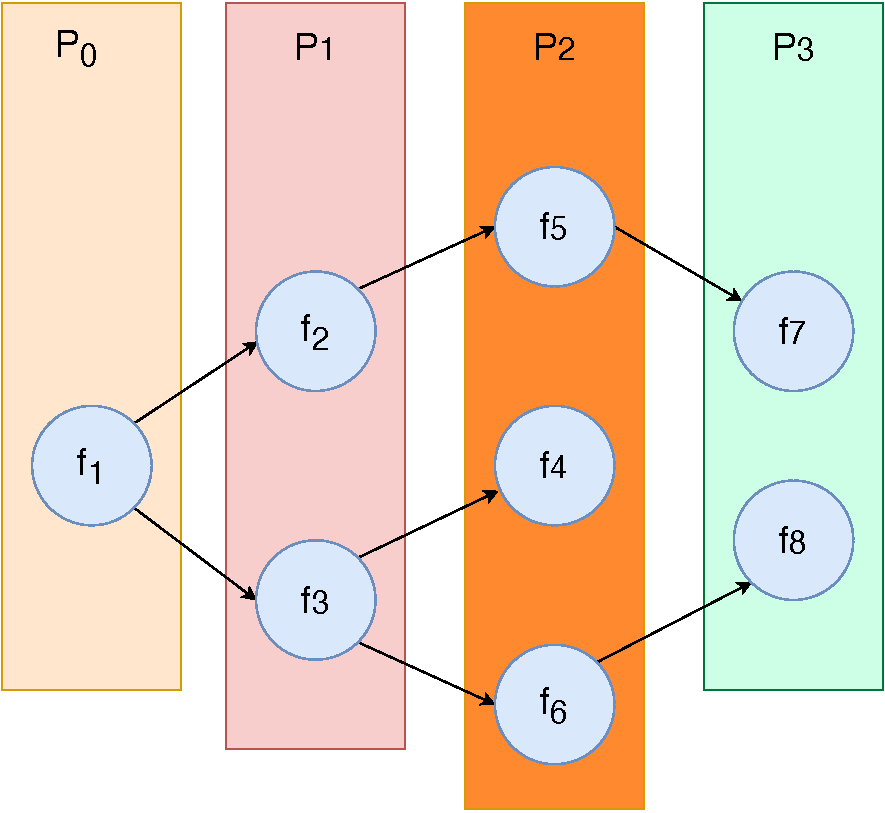
\includegraphics[height=0.8\textheight]{formalization_1.pdf}
\end{figure}
\end{frame}

\begin{frame}{Dependency Analysis: Formulation}
\begin{block}{Problem Formulation}
Suppose we have $G=\langle V, E\rangle$ and $V = P_0\cup P_1\cup \dots \cup P_m$\\
Where $P_0$ denotes the entry package of the analysed project.\\
Apparently, $P_0, P_1, \dots, P_m$ compose a partition of $V$.\\
Denote $D={f_k1,f_k2,\dots, f_kn}$, where $f_ki$ refers to a function that previously included in vulnerability database.\\
Find if " $\exists f_i\in P_0, f_j \in D \wedge f_i $ and $f_j$ is connected " holds.
\end{block}
\end{frame}


\begin{frame}{Dependency Analysis: Formalization}
\begin{figure}
    \centering
    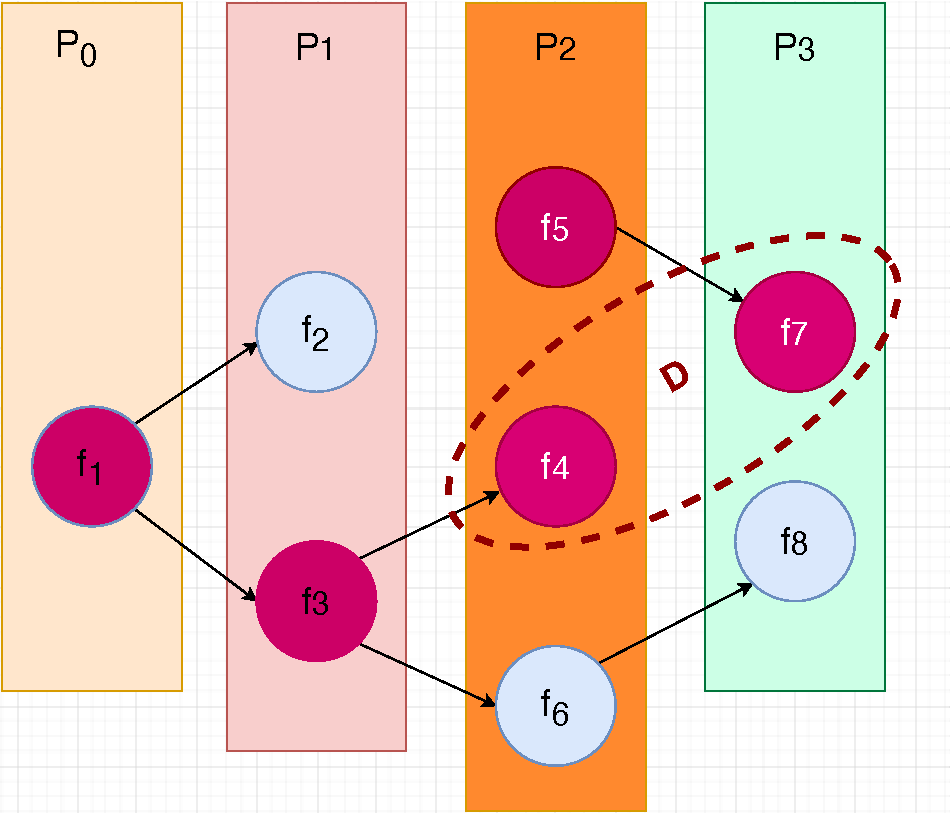
\includegraphics[height=0.8\textheight]{formalization.pdf}
\end{figure}
\end{frame}

%---------------------------------------------------------
\begin{frame}
\frametitle{Dependency Analysis: Obstacles}
The main obstacles of call graph generation are \textcolor{red}{Accuracy} and \textcolor{red}{Performance}. \\
To remedy these issues, optimizations are made under different scenarios. To name a few:
\begin{itemize}
    \item bundled JS with symbolic execution: Building Call Graphs for Embedded Client-Side Code in Dynamic Web Applications, FSE 14, Hung et al.
    \item bundled JS with test case generation: Slimming javascript applications: An approach for removing unused functions from javascript libraries, IST 19, Vázquez et al. 
    \item JS engine with test case generation: CodeAlchemist: Semantics-Aware Code Generation to Find Vulnerabilities in JavaScript Engines, NDSS 19, HyungSeok et al.
\end{itemize}
\end{frame}

\begin{frame}{Dependency Analysis: Sub-problems}
\begin{block}{$RQ_1$: How to Judge if $\langle f_i, f_j\rangle$ Exists?}
While such edge construction is well supported by techniques like AST in languages such as C/C++ and Java (e.g., through compiler IR), it is lacking for loosely typed language(e.g., JavaScript, Python). There for accuracy is always a problem for JavaScript Call Graph generation.
\end{block}
\end{frame}

\begin{frame}{Dependency Analysis: Sub-problems}
\begin{block}{$RQ_2$: How to Tell $f_i \in D$?}
Since package managers or repository service provider(e.g. GitHub) usually only give descriptive text on vulnerability of a package release. There exists work that try to aggregate structured data from JavaDocm with Machine Learning methods\footnote{On Using Machine Learning to Identify Knowledge in API Reference Documentation, arxiv 19, Davide et al.}. Yet, the accuracy are limited(79\%) and NPM documents are not semantically as good as JavaDoc. More structured descriptions on NPM \textbf{functions} or \textbf{APIs} are needed.
\end{block}
\end{frame}

\begin{frame}{Dependency Analysis: Sub-problems}
\begin{block}{$RQ_3$: How to Construct G within Reasonable Time?}
Although there's not a dependency analysis based on NPM call graph yet, such tasks under PYPI\footnote{Impact Analysis of Cross-Project Bugs on Software Ecosystems, ICSE 20, Wanwangying Ma et al.} and Java Libraries\footnote{An Empirical Study of Usages, Updates and Risks of Third-Party Libraries in Java Projects, arxiv 20, Ying Wang et al.} shows its time cost is non-ignorable.
\end{block}
\end{frame}

\begin{frame}{Conclusion \& Future Work}
This survey reports on prior conflicting analysis studies on NPM dependency ecosystem, highlighted and formalized the approach for a more concrete analysis. 
\begin{block}{First Phase: Call Graph Construction}
Compare and test different call graph construction methods on Express.js, and manually evaluate the results.
\end{block}
\end{frame}

\begin{frame}
\begin{figure}
    \centering
    
\includegraphics[width=0.9\textwidth]{thanks.pdf}
\end{figure}
\end{frame}
%---------------------------------------------------------

\end{document}